% intro 
The simulations of blood flows in nozzle, pump, and IVC with FEM and PFEM-2 are conducted and compared with experimental results in \cite{fda_res}, \cite{fda_nozzle}, \cite{fda_pump} and \cite{gallagher_exp}. The fluid is assumed to be Newtonian blood analog fluid. For the nozzle and pump flows, the fluid density and viscosity are $\rho= 1035$ kg/m\textsuperscript{3} and $\mu =3.5\times10^{-3}$ N-s/m\textsuperscript{2}, where as for the flow in IVC, the density and viscosity are $\rho=1817$ kg/m\textsuperscript{3}, $\mu=5.83\times10^{-3}$ N-s/m\textsuperscript{2} for resting condition and $\mu=5.49\times10^{-3}$ N-s/m\textsuperscript{2} for exercising condition. 

\subsection{Blood Nozzle}

%  nozzle intro
The simplified nozzle proposed by FDA consists of four parts containing characteristics of some blood-conveying medical devices. There are inlet and outlet tubes with diameter $0.012$ m, as well as a cone-shaped converging tube connecting the inlet tube with the nozzle throat with diameter $0.004$ m as shown in figure~\ref{fig:nozzlegeo1}. The flow experiences a gradual contraction of area from the inlet tube to the throat, then a sudden expansion of the area right after the throat to the outlet tube (figure~\ref{fig:nozzlegeo2}). It is set that the z coordinate along the axial direction has origin at the exit of the nozzle throat. The flow with Reynolds number $3500$ with flowrate $3.64\times10^{-5}$ m\textsuperscript{3}/s corresponding to turbulent flow regime is analyzed, where the Reynolds number is defined with the flow rate and the diameter at the throat. 

%% PEGGY: should these geometry figures be included?
\begin{figure}[htbp]
    \centering
    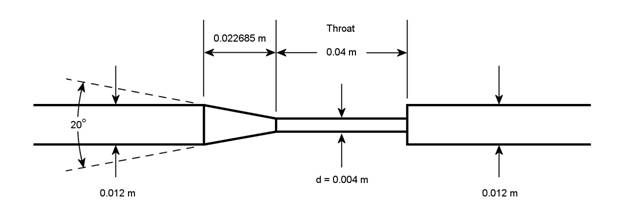
\includegraphics[width=3.2in]{imgs/nozzle_pump/nozzle_geo.jpg}
    \caption{The dimension of the idealized nozzle model proposed by FDA.}
    \label{fig:nozzlegeo1}
\end{figure}
\begin{figure}[htbp]
    \centering
    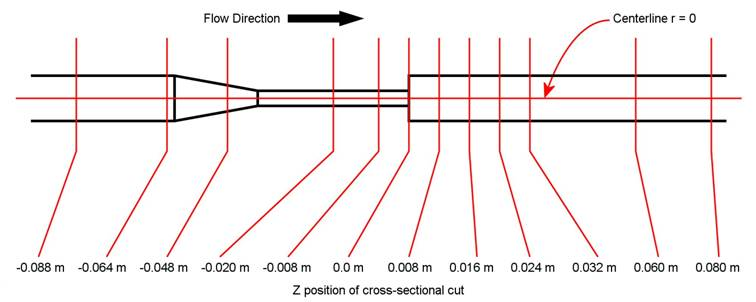
\includegraphics[width=3.2in]{imgs/nozzle_pump/nozzle_CS.jpg}
    \caption{The flow direction and the definition of the axial coordinate z.}
    \label{fig:nozzlegeo2}
\end{figure}


%  nozzle simulation setup
For the set up of the numerical simulation, the simulation domain starts from $z=-0.18$ m to $z=0.18$ m. The prescribed uniformly distributed velocity profile is imposed at the inlet while the pressure is constant at outlet. The Large Eddy Simulation (LES) Smagorinsky model is chosen to deal with the the turbulent flow regime in nozzle, and the Smagorinsky coefficient is set to be 0.1 empirically for flows in the pipe. The turbulence intensity is set to be $5$\% at the inlet. There are two different kinds of meshes considered in this study: mesh A with a more uniform mesh size in the outlet tube, and mesh B has a more refined mesh at certain area (figure~\ref{fig:nozzlemesh}). The mesh A has minimum mesh size $0.2$ mm and a total of $8.61$M elements. The mesh B has coarser meshes in the outlet tube than mesh A, but has mesh refinement near the exit of the throat. The minimum mesh size of mesh B is $0.1$ mm with total of $1.13$M elements. The purpose of using two distinct meshes is for the observation of the influence of mesh on FEM and PFEM-2. Simulations with different CFL number will also be done to examine the influence of time step size with these two methods.

\begin{figure}[htbp]
    \centering
    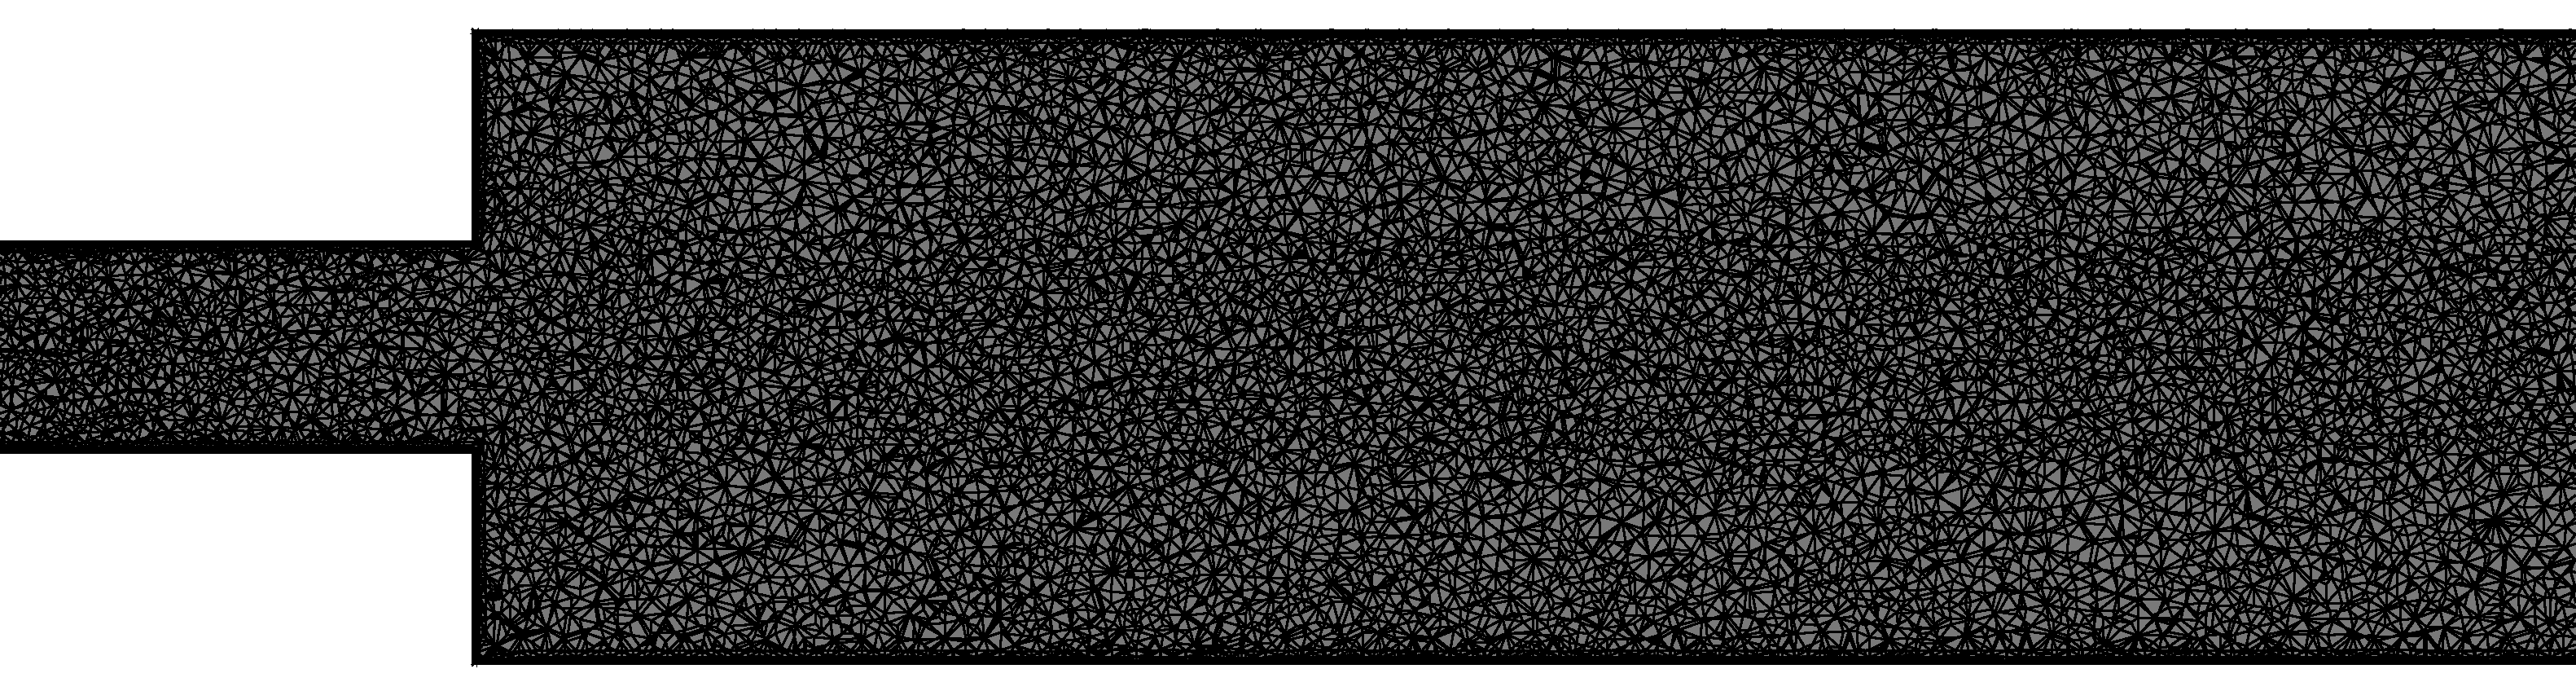
\includegraphics[width=3.2in]{imgs/nozzle_pump/nozzle_fmesh.pdf}
    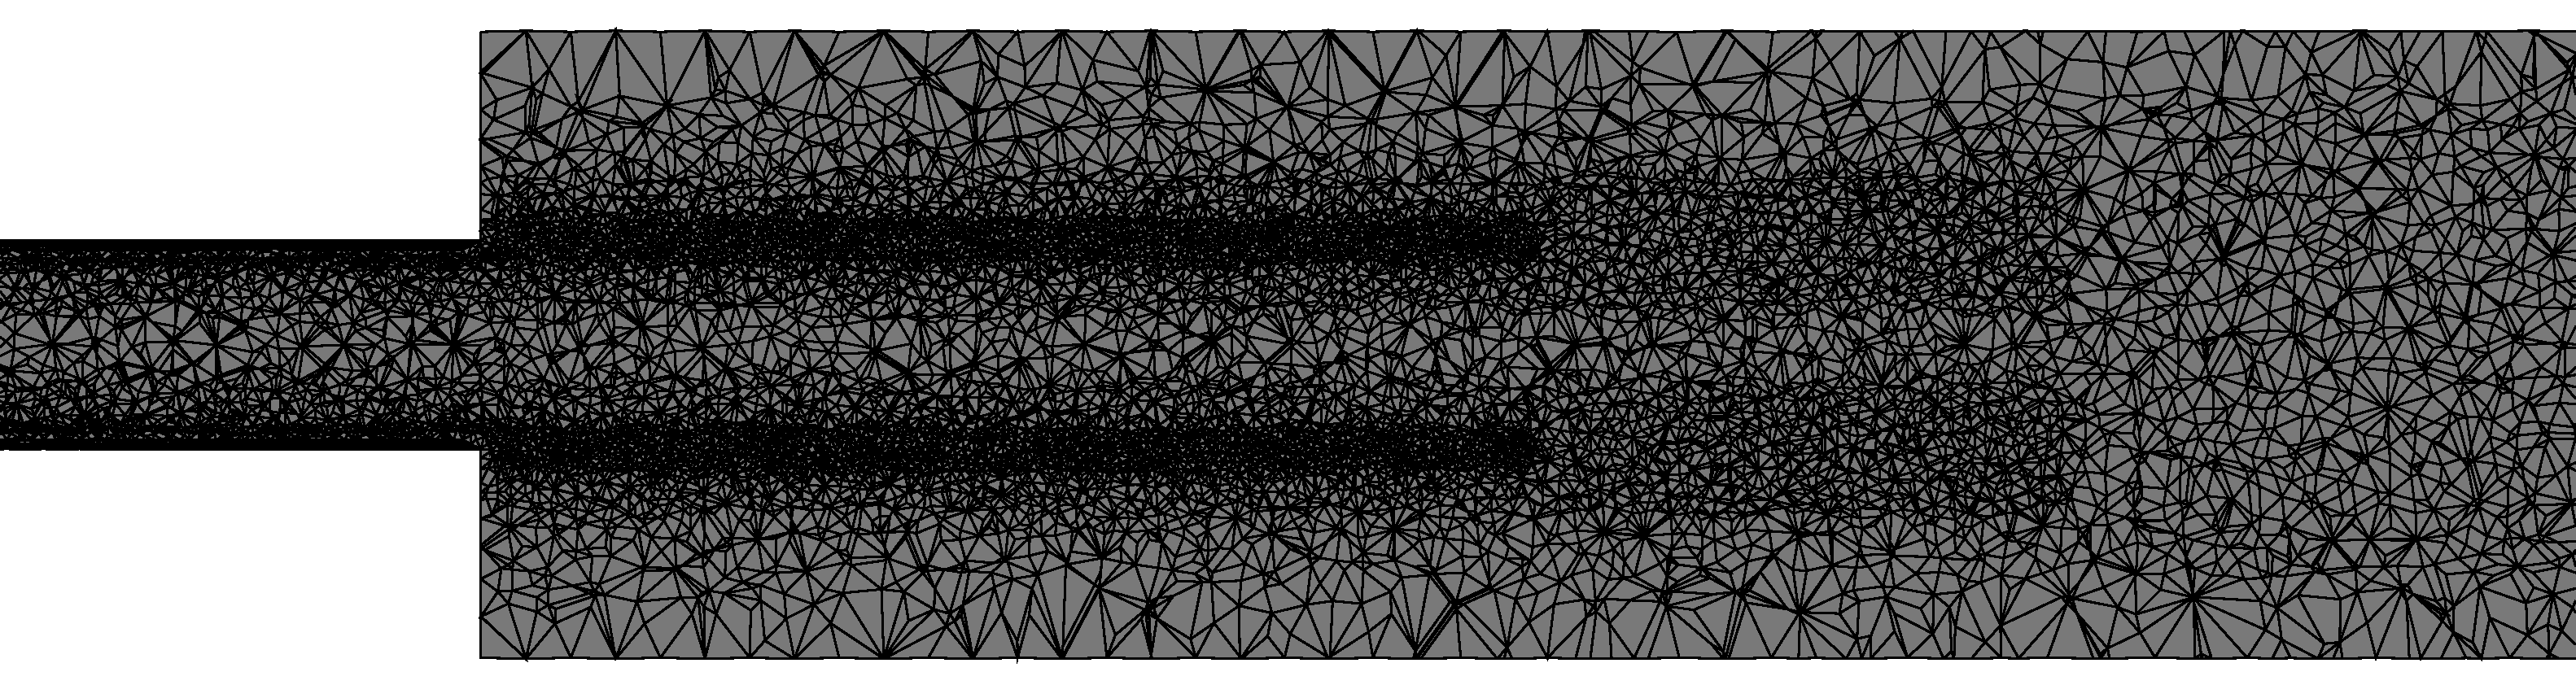
\includegraphics[width=3.2in]{imgs/nozzle_pump/nozzle_pmesh.pdf}
    \caption{The two meshes A (top) and B (bottom) used in the blood nozzle simulations.}
    \label{fig:nozzlemesh}
\end{figure}

% nozzle result and analysis

The distributions of velocity magnitude in the nozzle after reaching steady state are shown in figure \ref{fig:nozzlevelfm} and \ref{fig:nozzlevelpm}. It can be observed that the sudden expansion at the exit of the throat leads to the formation of a jet. In the turbulent regime, the center velocity of jet has a sudden decrease called jet breakdown. Most of the results show the breakdown of the jet, but with different breakdown locations. This can be shown clearly in figure~\ref{fig:nozzlemidvel} depicting the velocity along the center line of the nozzle, where the origin of the axial coordinate is at the exit of the throat (figure~\ref{fig:nozzlegeo2}). It can be observed that the results by PFEM-2 have good agreement with experimental result by \cite{hariharan_nozzle} with both meshes. Also, the results using PFEM-2 is not affected much by the time step size, since the convection terms is taken care of separately. However, for the results using FEM, it can be affected largely once CFL number is larger than 1. Also, the breakdown locations are also affected by the mesh configuration. \textbf{CHECK}*** This may be due to the additional viscosity added through the convection stabilization term in this FEM algorithm.***

\begin{figure}[htbp]
    \centering
    FEM\\
    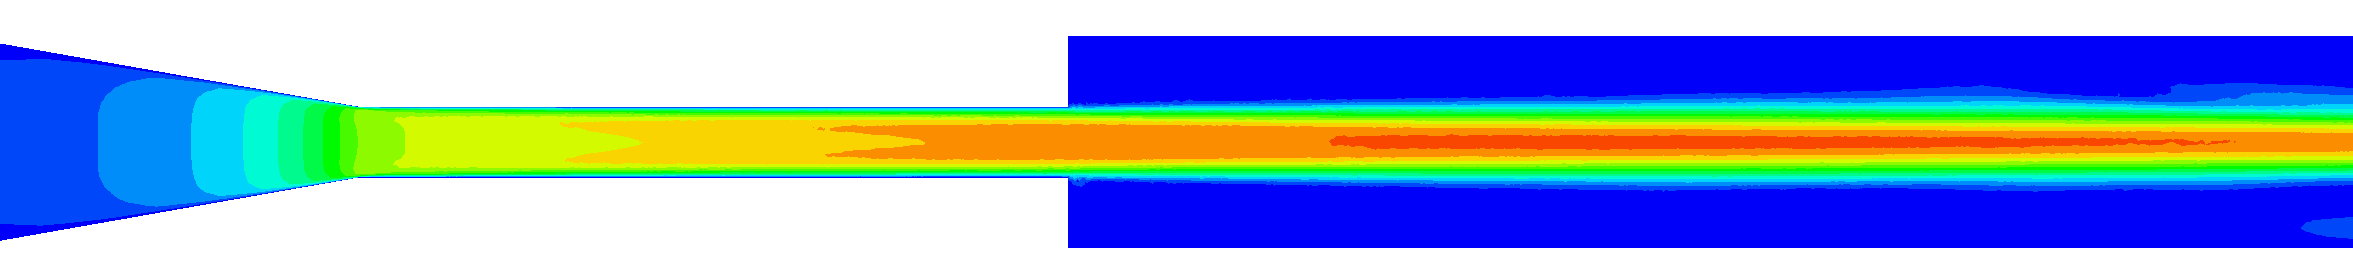
\includegraphics[width=3.2in]{imgs/nozzle_pump/nozzle_fem_fm_cfl1.png}
    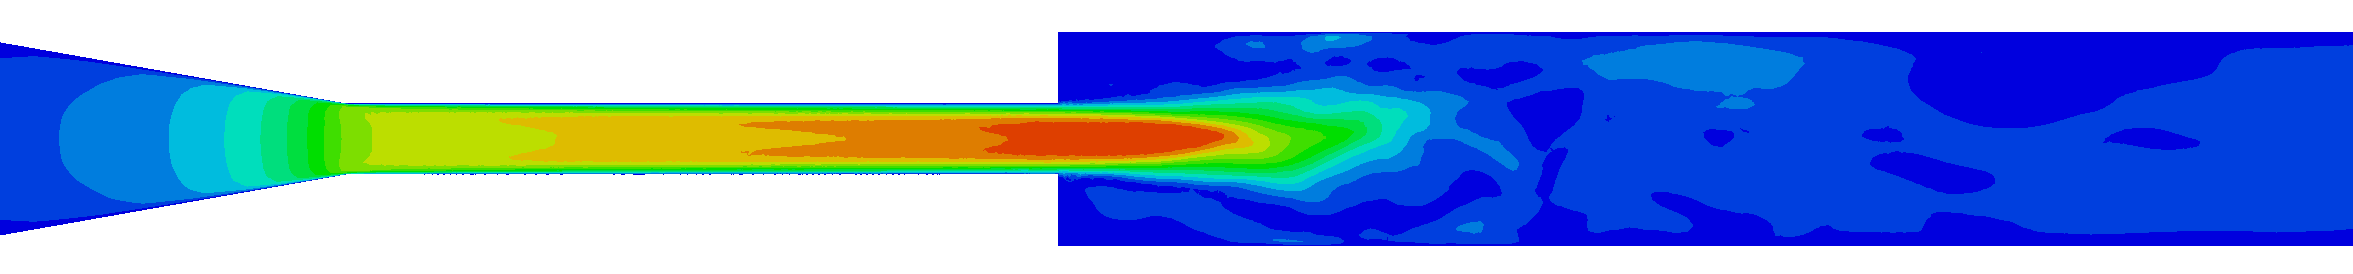
\includegraphics[width=3.2in]{imgs/nozzle_pump/nozzle_fem_fm_cfl5.png}\\
    PFEM-2\\
    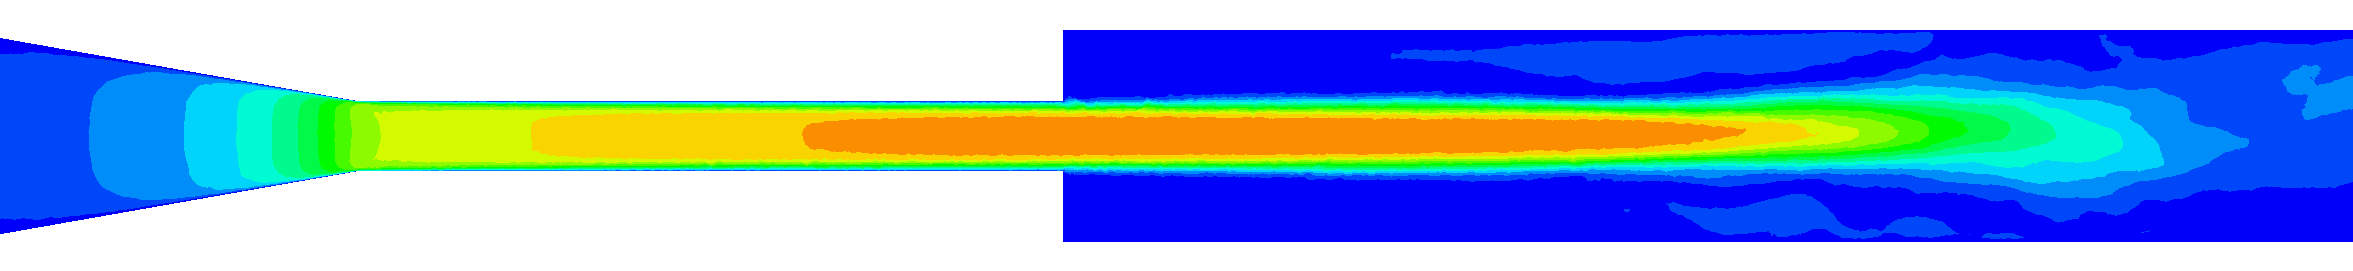
\includegraphics[width=3.2in]{imgs/nozzle_pump/nozzle_pfem_fm_cfl1.png}
    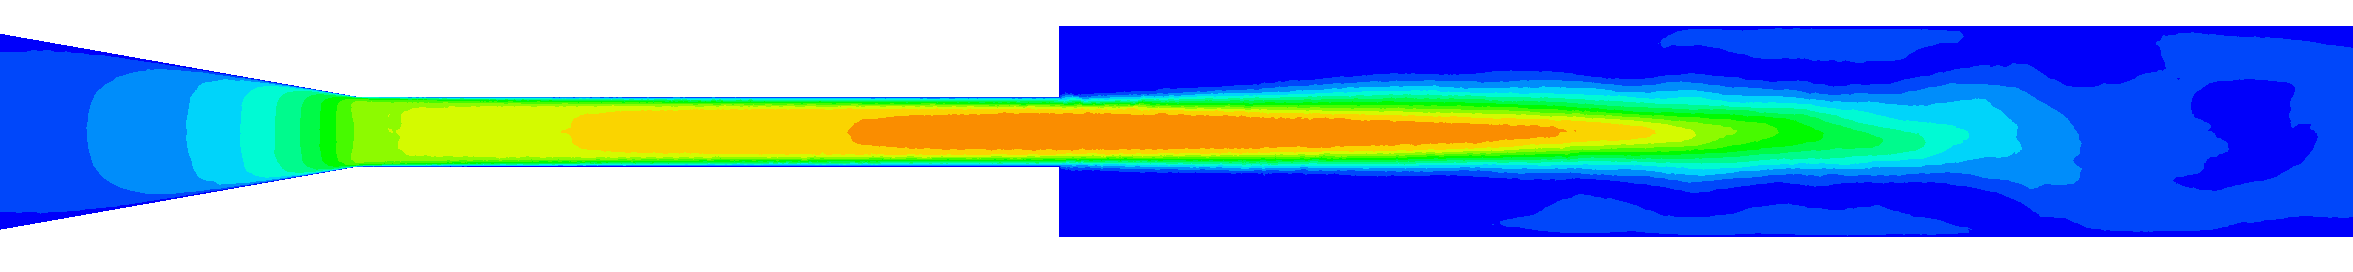
\includegraphics[width=3.2in]{imgs/nozzle_pump/nozzle_pfem_fm_cfl5.png}
    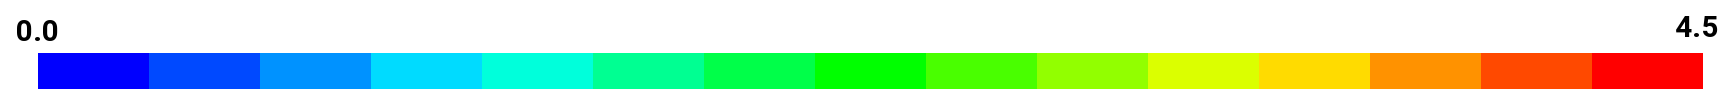
\includegraphics[width=3.2in]{imgs/nozzle_pump/nozzle_legend.png}
    \caption{The magnitude of velocity field at steady state with mesh A using FEM and PFEM-2 with CFL number equals to 1 (1st and 3rd plots) and 5 (2nd and 4th plots). }
    \label{fig:nozzlevelfm}
\end{figure}

\begin{figure}[htbp]
    \centering
    FEM\\
    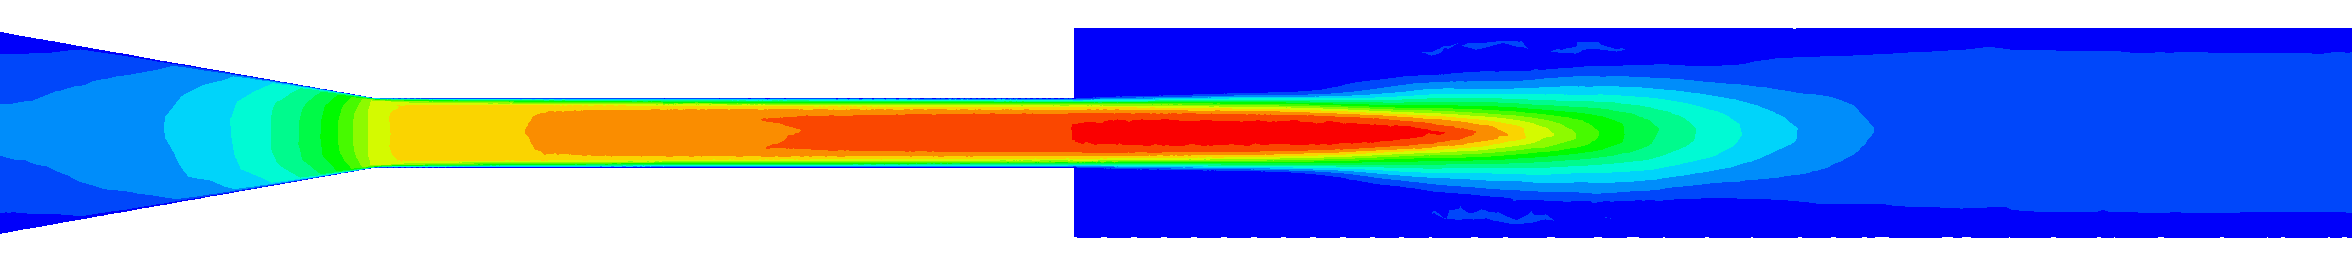
\includegraphics[width=3.2in]{imgs/nozzle_pump/nozzle_fem_pm_cfl1.png}
    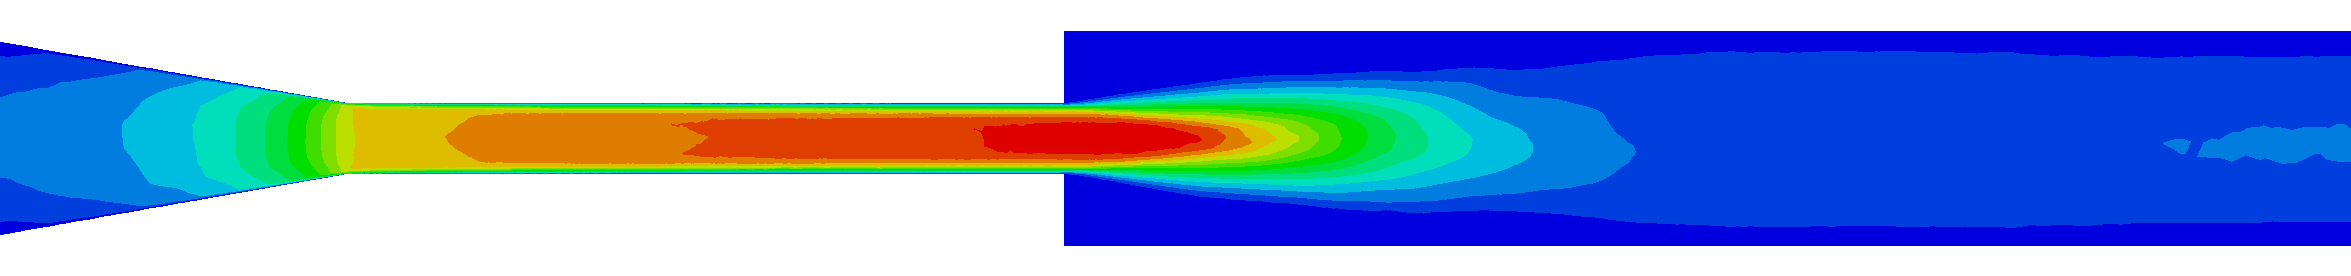
\includegraphics[width=3.2in]{imgs/nozzle_pump/nozzle_fem_pm_cfl10.png}
    PFEM-2\\
    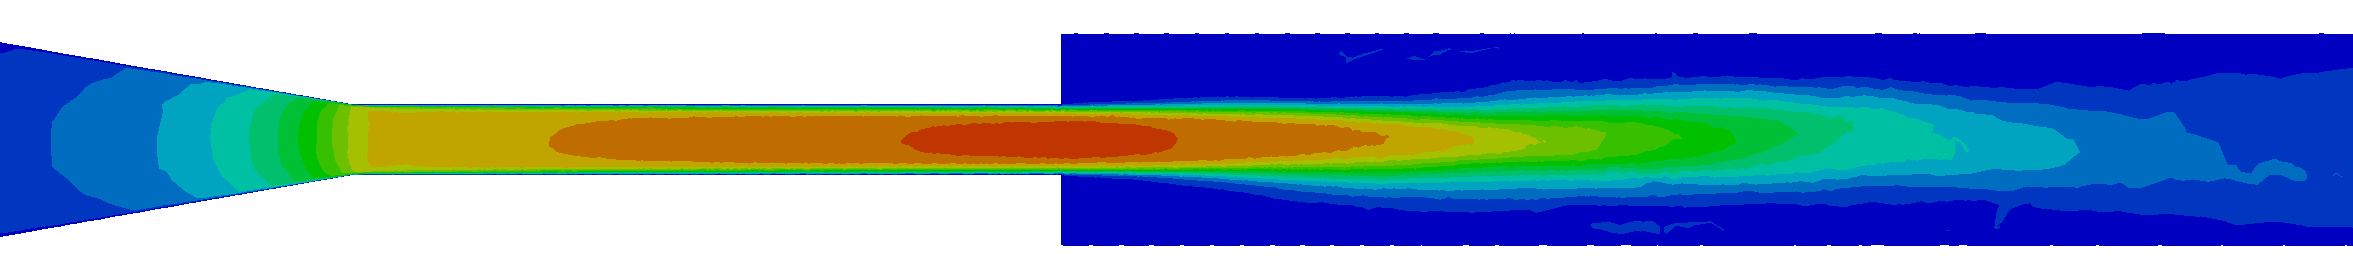
\includegraphics[width=3.2in]{imgs/nozzle_pump/nozzle_pfem_pm_cfl1.png}
    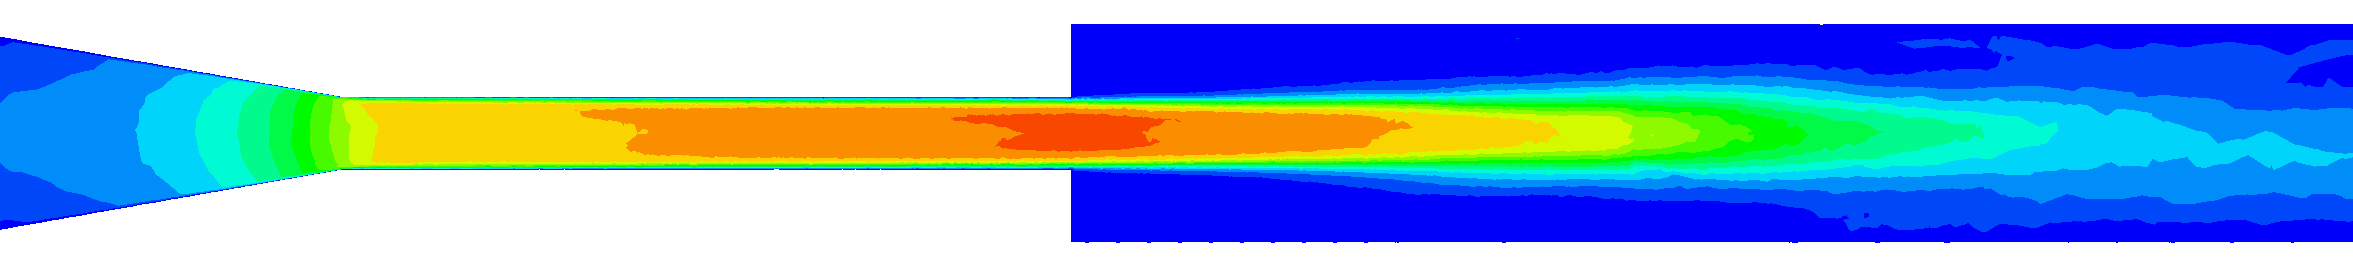
\includegraphics[width=3.2in]{imgs/nozzle_pump/nozzle_pfem_pm_cfl10.png}
    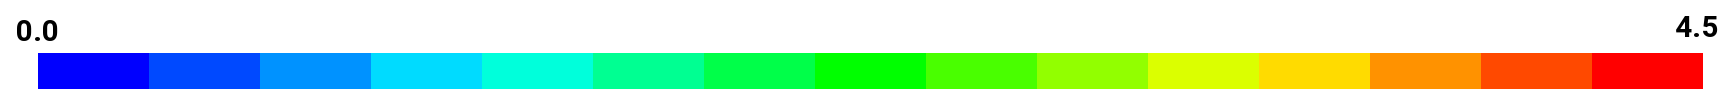
\includegraphics[width=3.2in]{imgs/nozzle_pump/nozzle_legend.png}
    \caption{The magnitude of velocity field at steady state with mesh B using FEM and PFEM-2 with CFL number equals to 1 (1st and 3rd plots) and 10 (2nd and 4th plots).}
    \label{fig:nozzlevelpm}
\end{figure}


\begin{figure}[htbp]
    \centering
    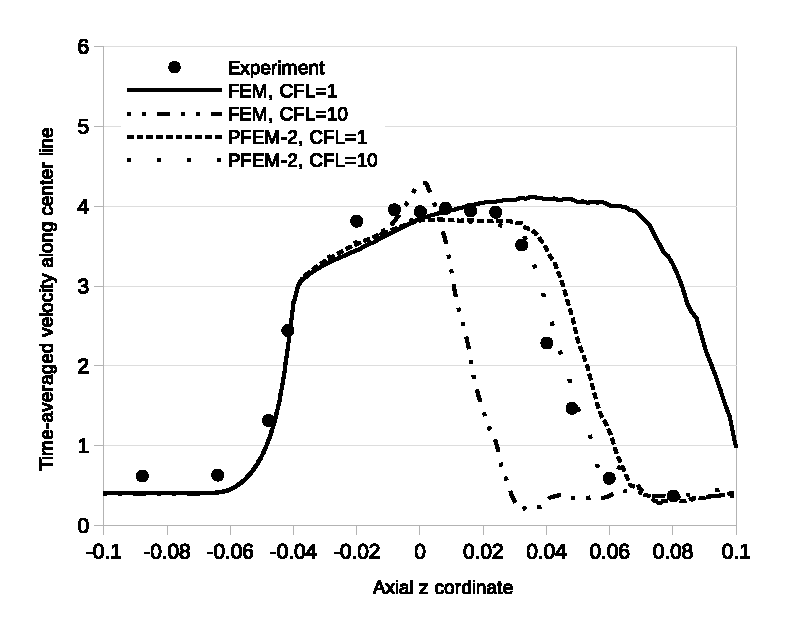
\includegraphics[width=3.2in]{imgs/nozzle_pump/nozzle_midvel_fm2.eps}
    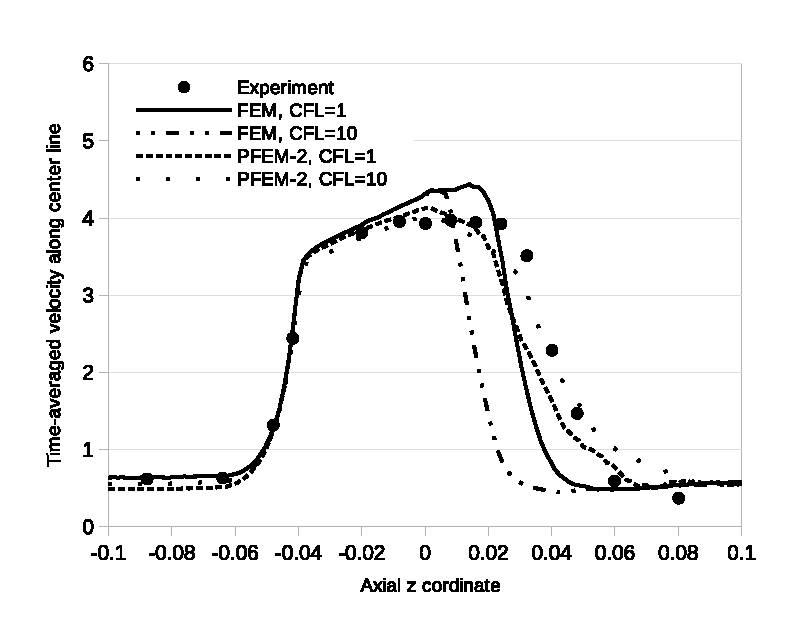
\includegraphics[width=3.2in]{imgs/nozzle_pump/nozzle_midvel_pm2.eps}
    \caption{The distribution of the axial velocity in the nozzle along the center line. The top figure depicts the results with mesh A (top) and mesh B (bottom).
%The distribution of the axial velocity in the nozzle along the center line. The top figure depicts the results with mesh A using FEM and CFL=1 (solid), FEM and CFL=5 (dash-dotted), PFEM-2 and CFL=1 (dashed) and PFEM2 and CFL=5 (dotted). The bottom figure depicts the results with mesh B using FEM and CFL=1 (solid), FEM and CFL=10 (dash-dotted), PFEM-2 and CFL=1 (dashed) and PFEM2 and CFL=10 (dotted).
}
    \label{fig:nozzlemidvel}
\end{figure}

\subsection{Blood Pump}

%  pump intro
The geometry of the simplified centrifugal pump is shown in the figure~\ref{fig:pumpgeo}. The flow enters the chamber through a curved tube with diameter $12$ mm. The diameter of the inner chamber of the housing is $60$ mm and the thickness is $9$ mm. The rotor inside the chamber is with diameter $52$ mm and $4$ mm thick, along with four $3$ mm thick straight blades. The chamber is connected with a throat at its outlet, followed by a diffuser to the outlet tube with diameter $12$ mm. The pump flow with flowrate $Q = 6$ L/min and rotational speed $3500$ RPM is simulated. 

%% PEGGY: should these geometry figures be included?
\begin{figure}[htbp]
    \centering
    \begin{minipage}[c][2.5in][c]{0.9\linewidth}
        \centering
        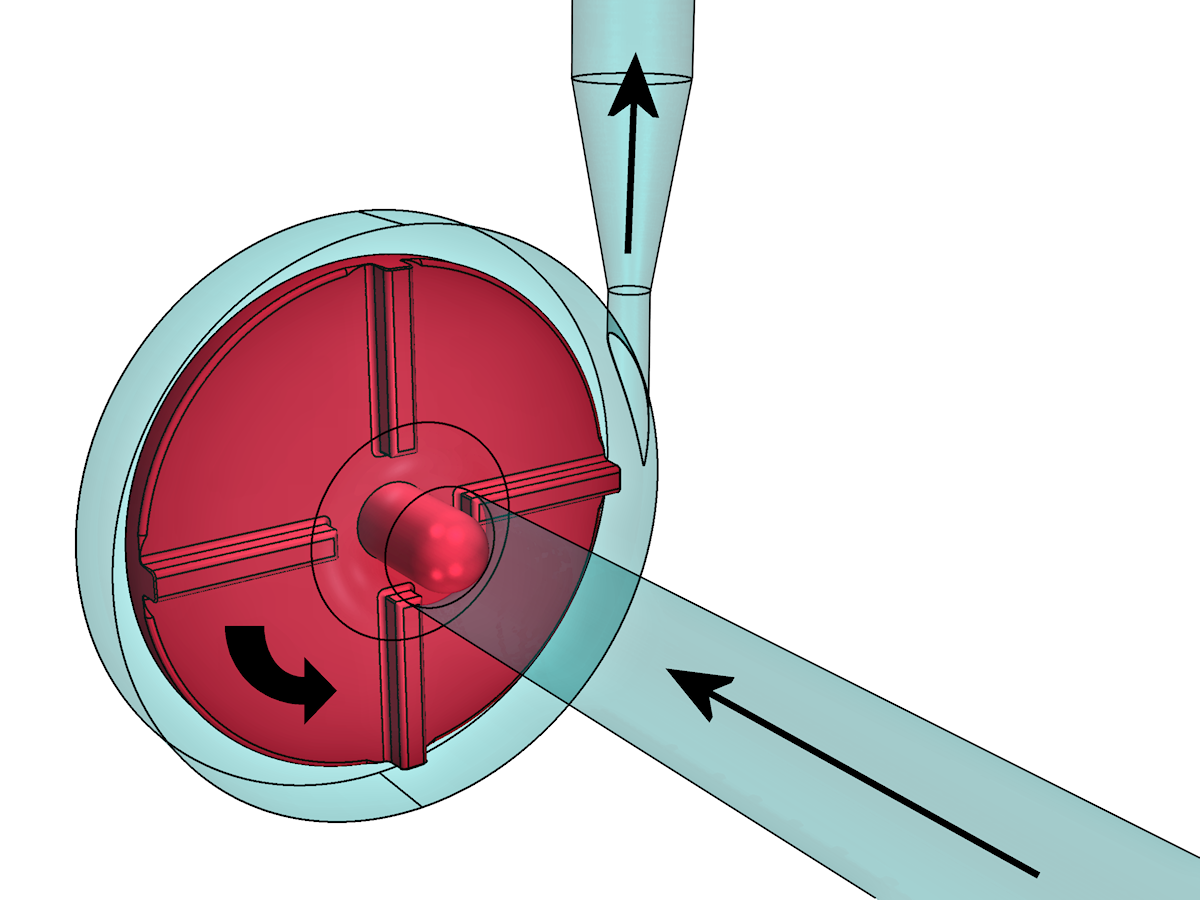
\includegraphics[width=3.2in]{imgs/nozzle_pump/housing_and_rotor.png}
    \end{minipage}
    \begin{minipage}[c][2.5in][c]{0.9\linewidth}
        \centering
        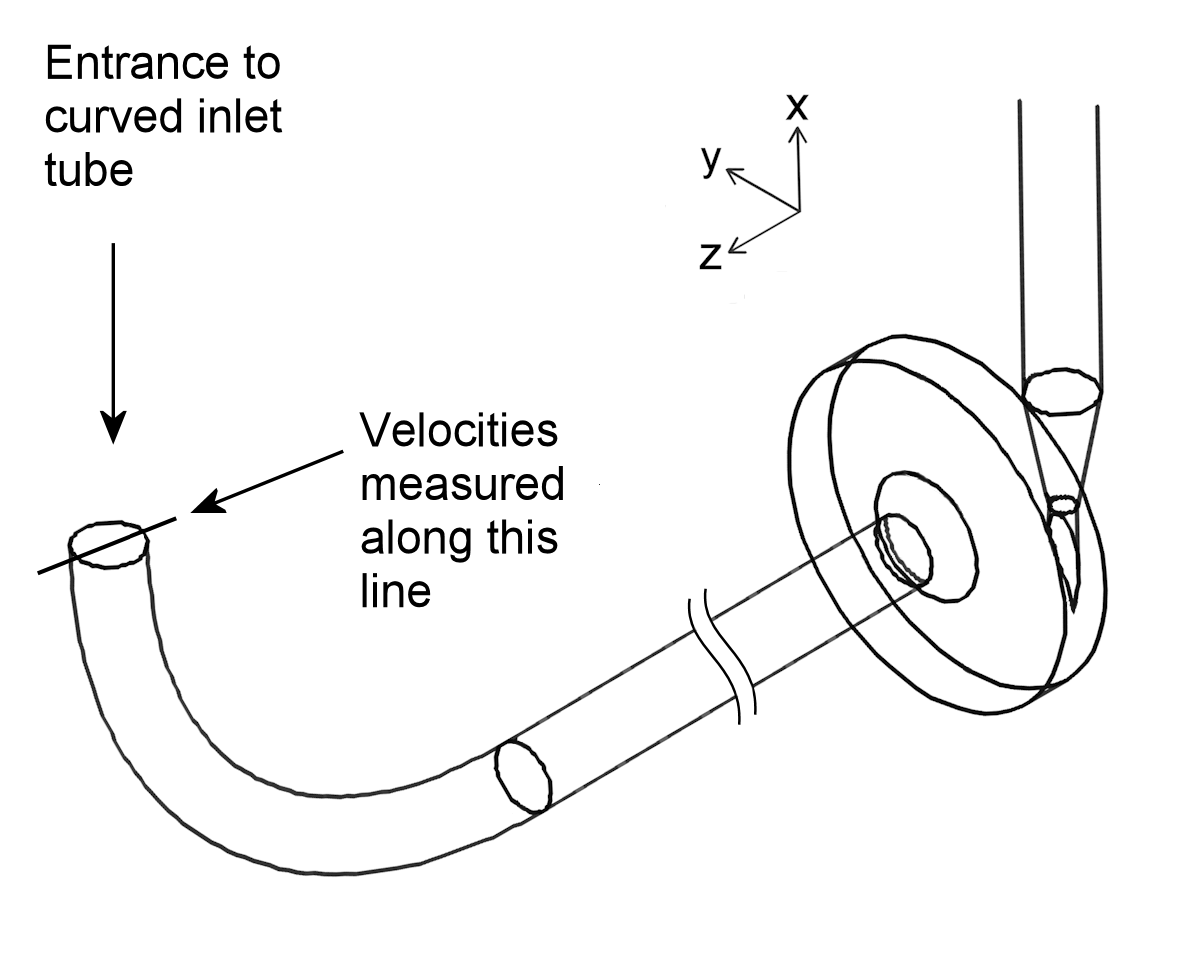
\includegraphics[width=3.2in]{imgs/nozzle_pump/inlet_velcocity_profile_location.png}
    \end{minipage}
    \caption{The geometry of and the flow direction in the blood pump (top), and the location where the velocity is measured in the experiments the velocity profile is prescribed in the simulations (right).}
    \label{fig:pumpgeo}
\end{figure}

%  pump simulation setup
As to the simulation set up, the velocity distribution is prescribed at the inlet (see figure~\ref{fig:pumpgeo} bottom plot), where the velocity profiles are obtained from the experimental measurements using PIV from \cite{cpi}. The pressure at the outlet is set to be constant, and the gravitational force is included. Since the goal is to predict the flow field after it reaching steady state, instead of letting the rotor rotate during simulation, the non-inertial reference frame is applied on the fluid around the rotor. This is because the flow around the rotor at steady state can be analogue to flow experiencing constant angular velocity. Using non-inertial reference frame avoids mesh distortion and frequent remeshing due to rotation. For turbulence model, the LES Wall-Adapting Local Eddy-viscosity (WALE) model is employed, with 7\% of turbulence intensity imposed at the inlet. 

The simulation domain is decomposed into around 1 million tetrahedron elements. The mesh size is $0.5$ mm on the rotor blades and $0.3$ mm at the outlet of the chamber to diffuser. The mesh is locally refined around the throat as shown in figure~\ref{fig:pumpmesh}. The simulation result is obtained after $15$ rotations of the rotor, when the pump flow already reaches steady state. The time step size is around $10^{-5}$ s in FEM and PFEM-2 simulations at steady state so that the CFL number is less or equal than $1$.  

\begin{figure}[htbp]
    \centering
    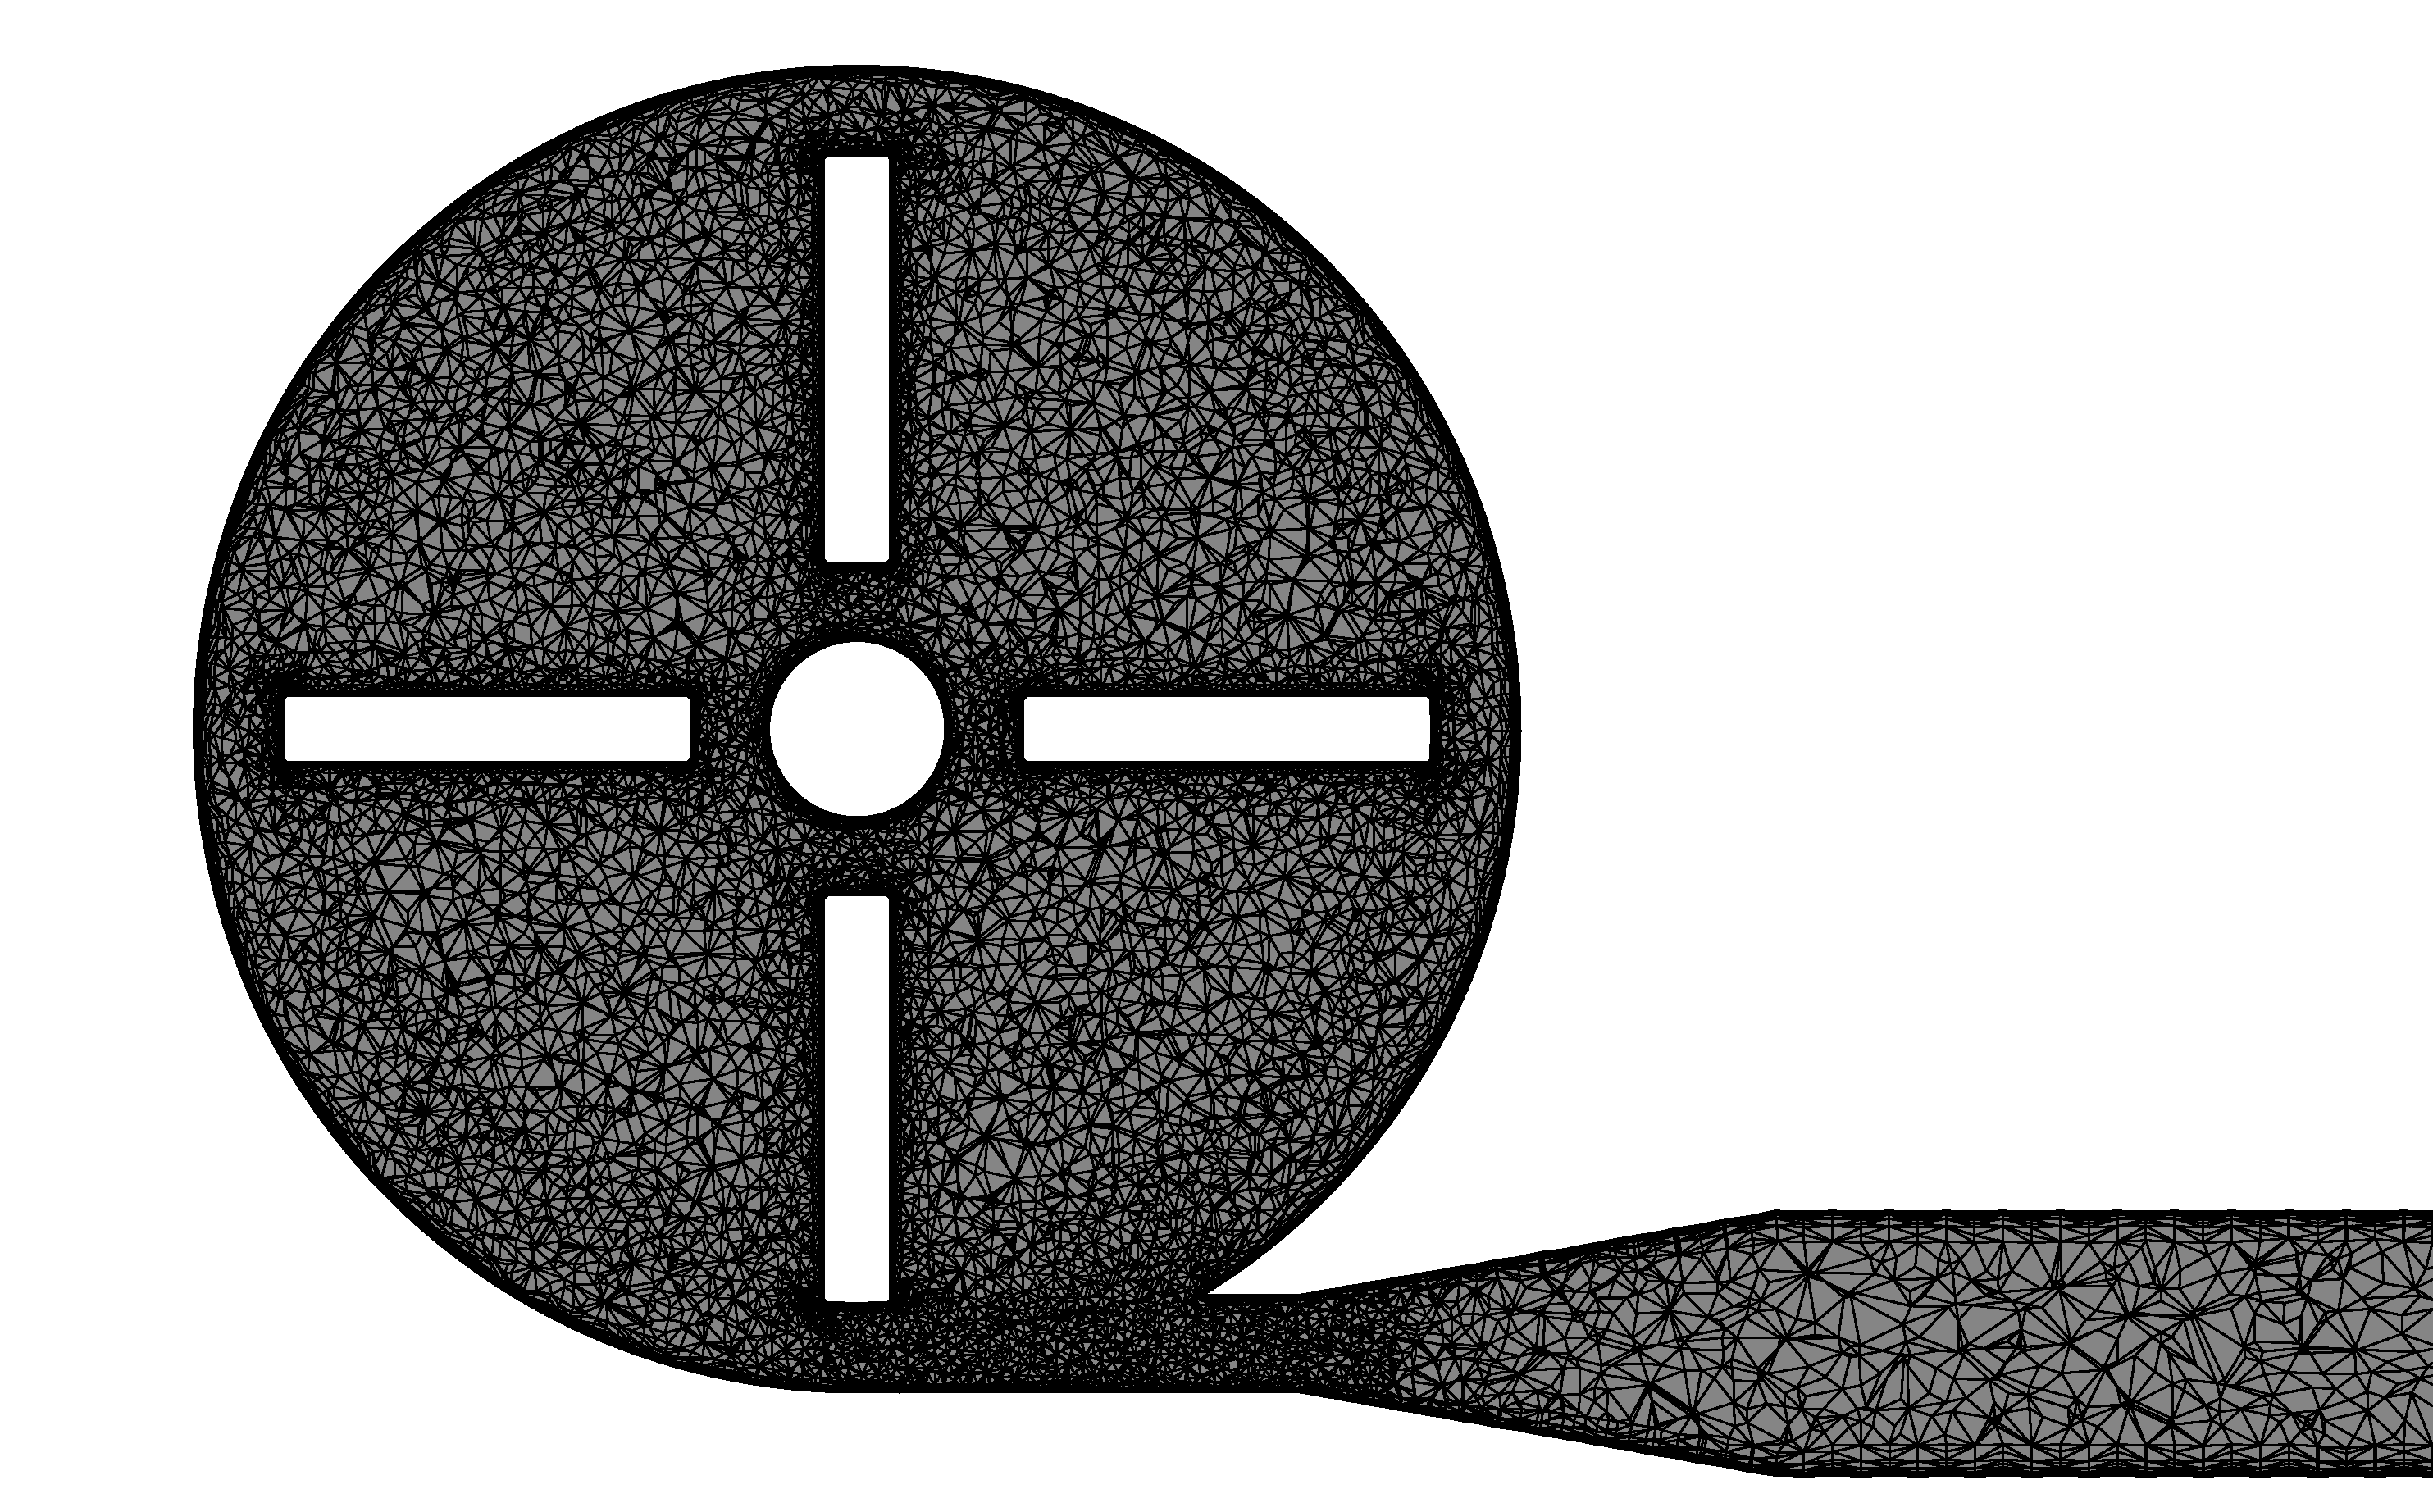
\includegraphics[width=3in]{imgs/nozzle_pump/pump_mesh.pdf}
    \caption{The mesh configuration used in the pump flow simulation on the plane which coincides to the mid-axis plane of the outlet diffuser.}
    \label{fig:pumpmesh}
\end{figure}

% pump result & analysis

The obtained pressure difference across the pump by experiment and simulations are listed in table~\ref{tab:pumppres}. Using FEM the discrepancy with experiment is only $3.6$\%. On the other hand, PFEM-2 predicts a much higher pressure difference. From the distribution of the velocity and pressure fields in the chamber (figure \ref{fig:pumpvel} and \ref{fig:pumppres}, it can be observed that the velocity pattern obtained with PFEM-2 is different from FEM. With PFEM-2, the velocity is higher mainly in front of the leading edge of the blade, where with FEM, the velocity is higher at both side of the blade, but more near the trailing edge. \textbf{CHECK:} ***This might due to in the present PFEM-2 method, the convection and viscous effect are treated separately and sequentially, and an explicit integration scheme is employed. As a result, the particles pushed by the rotor blades have less tendency to turn in chamber using PFEM-2 than FEM, which can be observed from the streamline plot in figure~\ref{fig:pumpsl}. This leads to a larger pressure gradient in the radial direction to make particles turn in the chamber. ***

\begin{table}[h]
\caption {The pressure differences across the pump.}\label{tab:pumppres} 
\centering
\begin{tabular}{|c|c|}
\hline
 & Pressure (mmHg) \\ \hline
Experiment \cite{mali_cfd}    & 272.38    \\ \hline
FEM    & 282.40             \\ \hline
PFEM-2    & 489.64          \\ \hline
\end{tabular}
\end{table}

\begin{figure}[htbp]
    \centering
    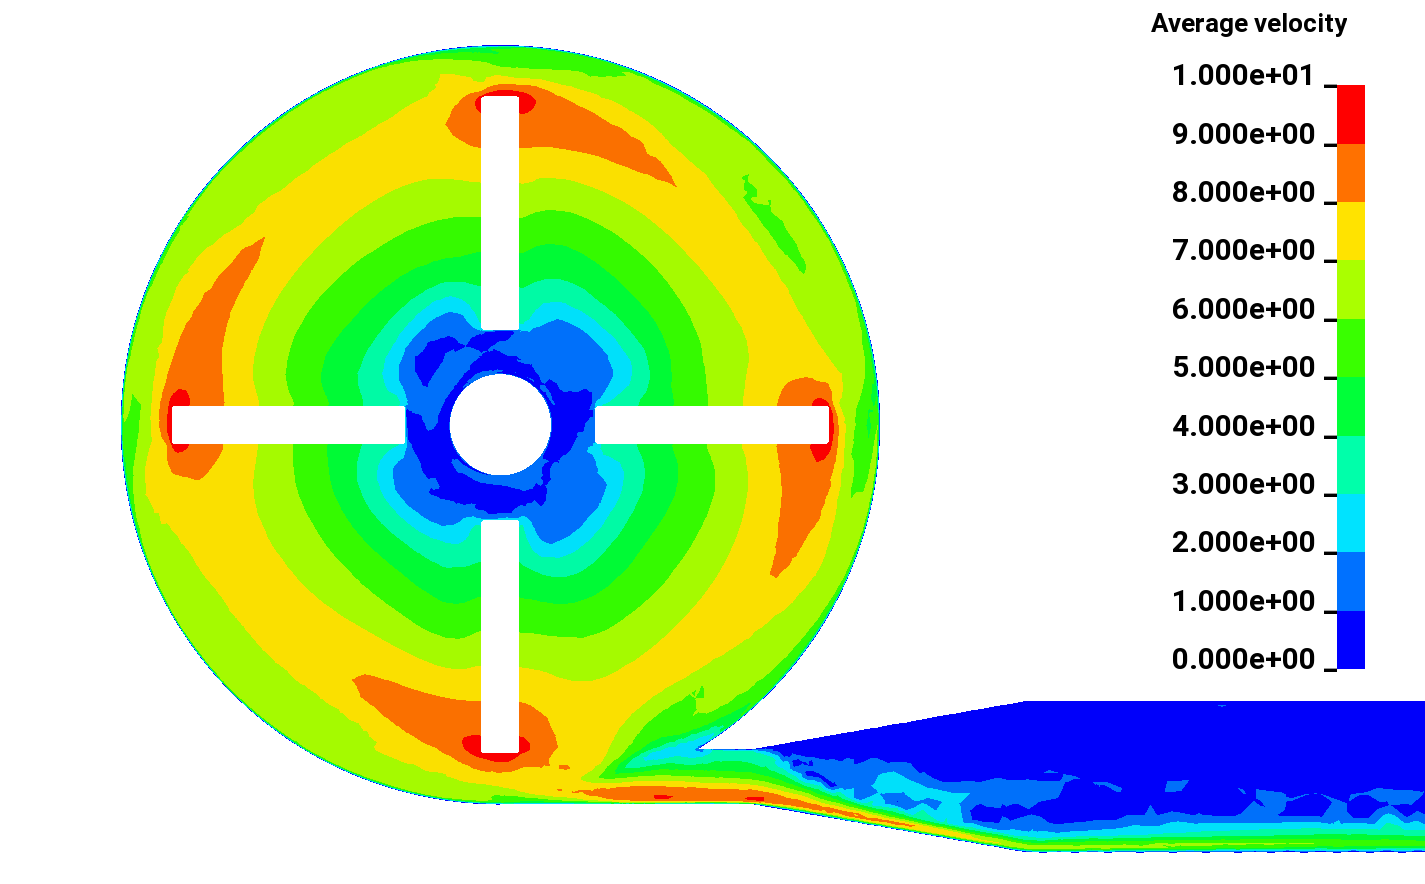
\includegraphics[width=3in]{imgs/nozzle_pump/pumpvel_fem.png}\\
    \vspace{.5cm}
    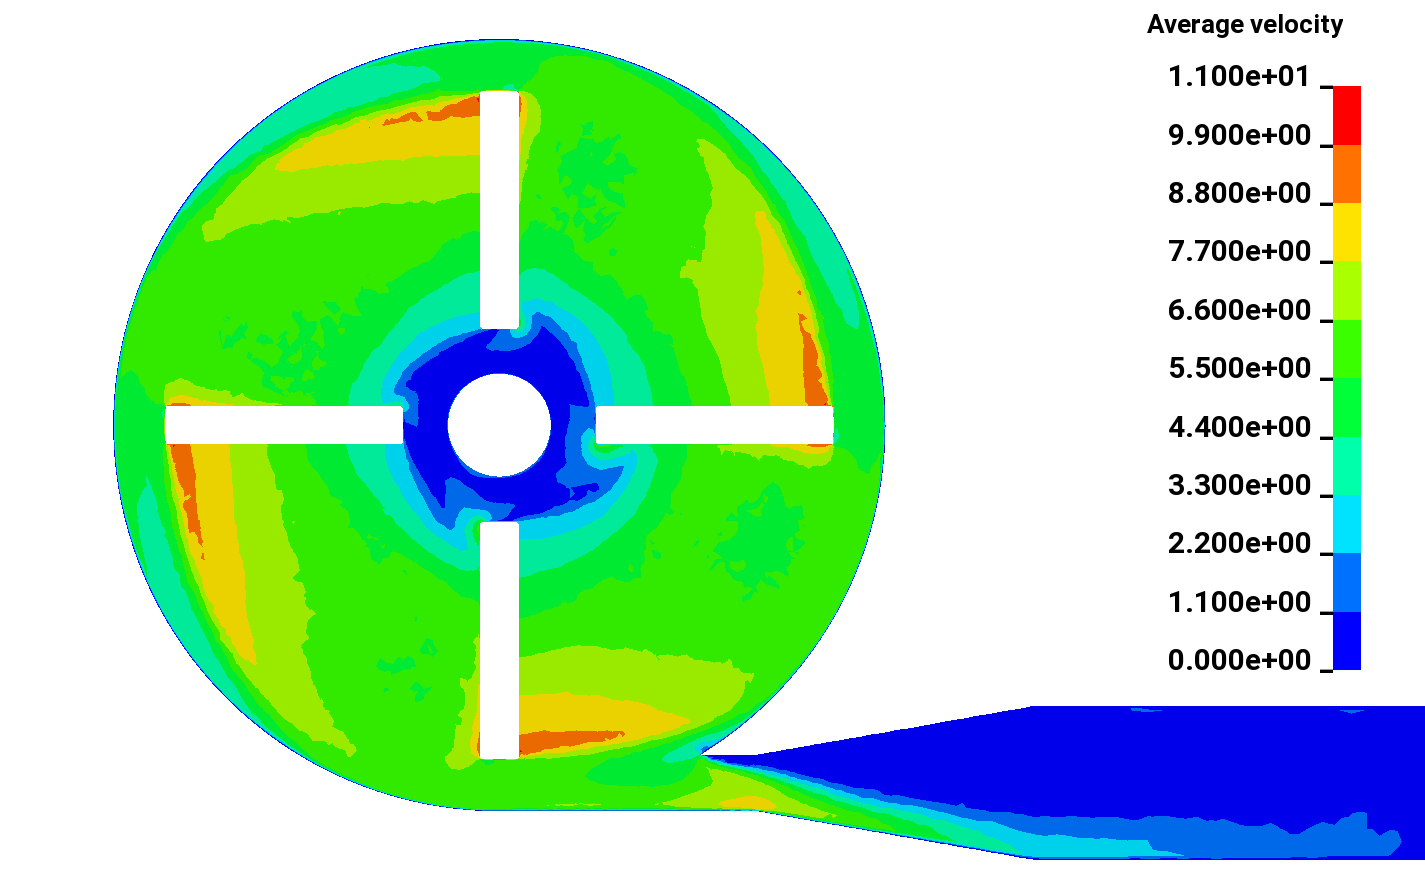
\includegraphics[width=3in]{imgs/nozzle_pump/pumpvel_pfem.png}
    \caption{The magnitude of velocity distribution on the plane which coincides to the mid-axis plane of the outlet diffuser using FEM (top) and PFEM-2 (bottom).}
    \label{fig:pumpvel}
\end{figure}

\begin{figure}[htbp]
    \centering
    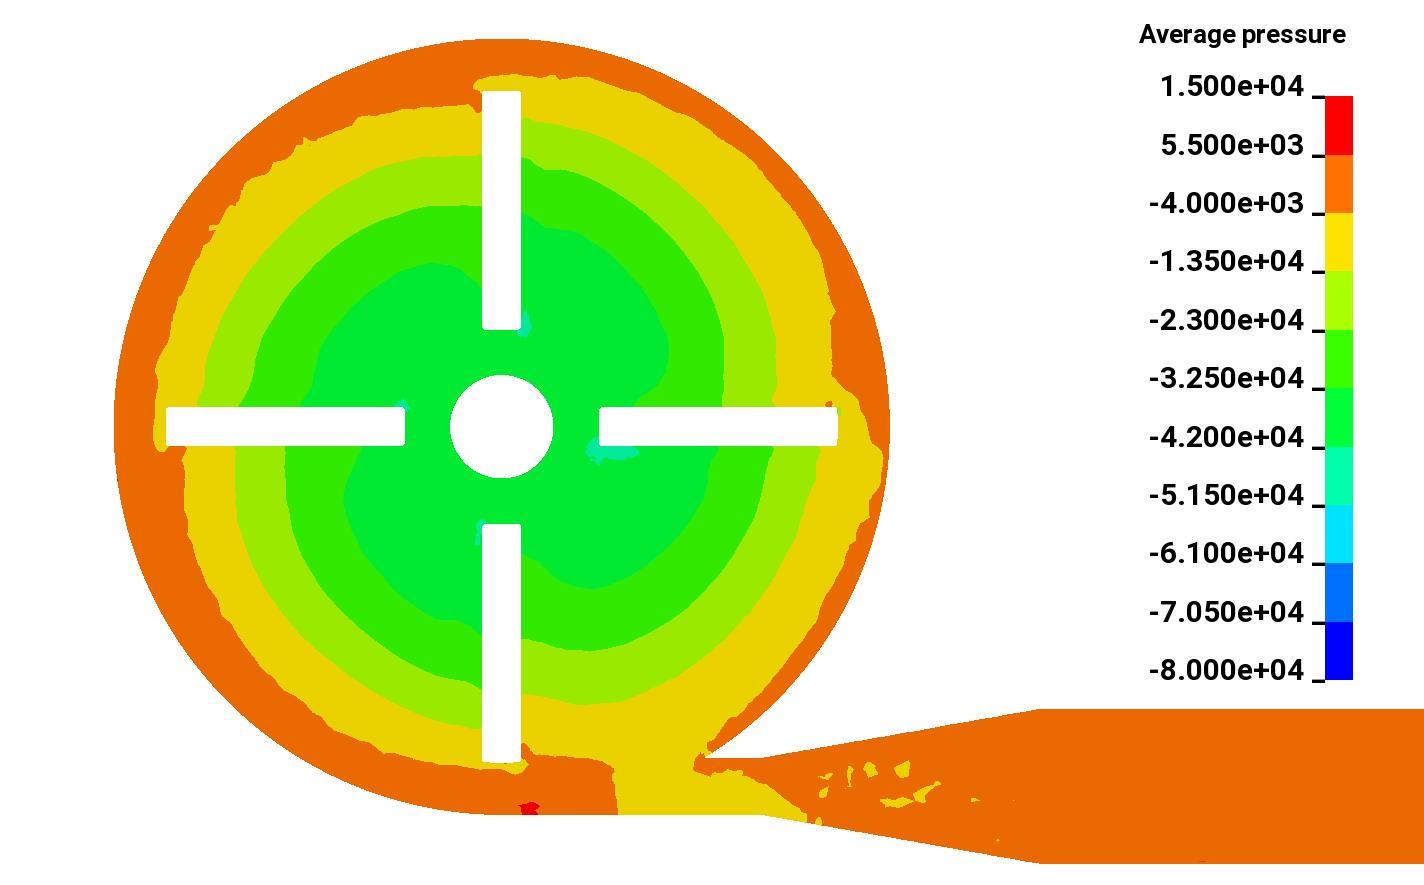
\includegraphics[width=3in]{imgs/nozzle_pump/pumppres_fem.png}\\
    \vspace{.5cm}
    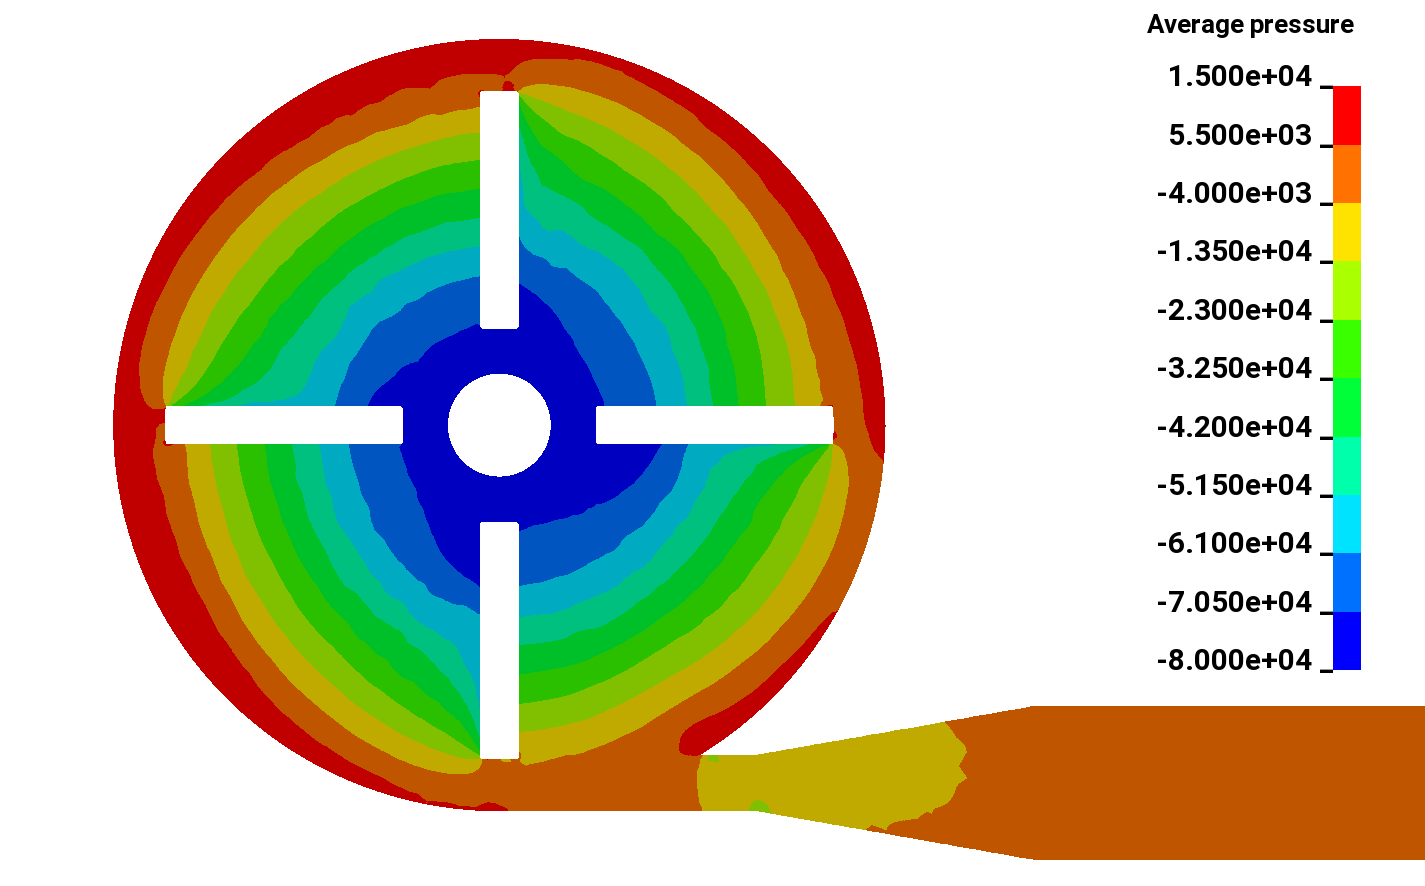
\includegraphics[width=3in]{imgs/nozzle_pump/pumppres_pfem.png}
    \caption{The pressure distribution on the plane which coincides to the mid-axis plane of the outlet diffuser using FEM (top) and PFEM-2 (bottom).}
    \label{fig:pumppres}
\end{figure}

\begin{figure}[htbp]
    \centering
    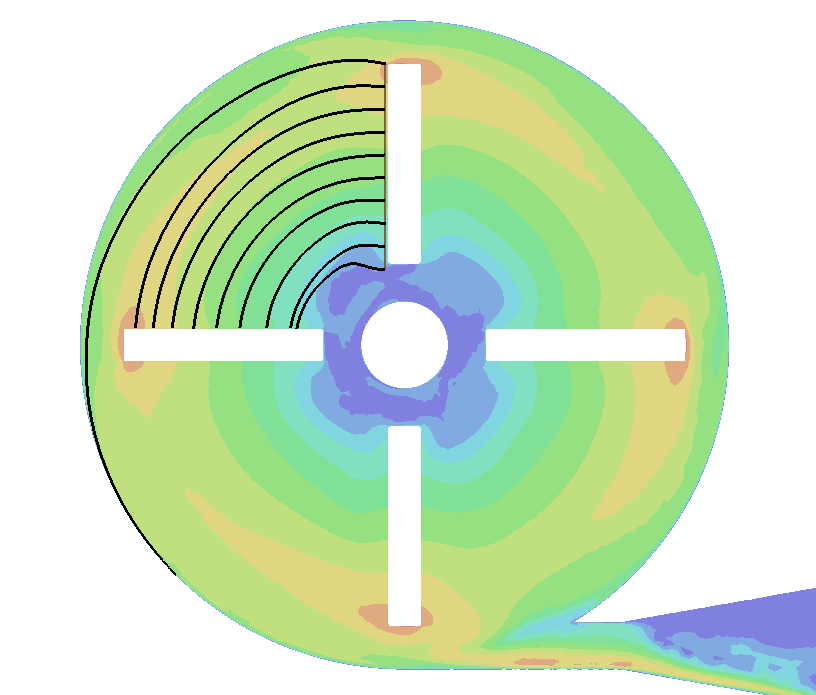
\includegraphics[width=2.2in]{imgs/nozzle_pump/pump_sl_fem.png}\\
    \vspace{.5cm}
    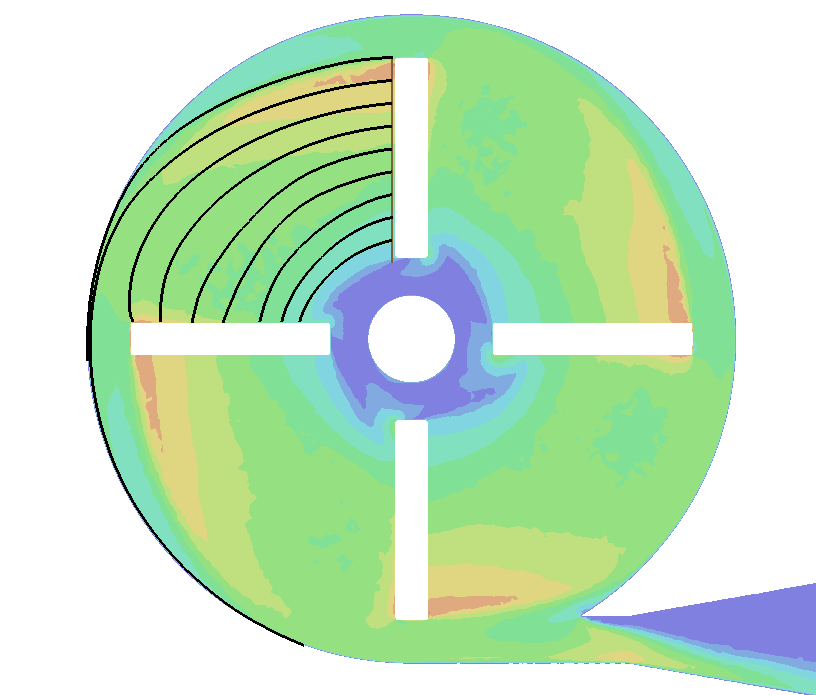
\includegraphics[width=2.2in]{imgs/nozzle_pump/pump_sl_pfem.png}
    \caption{The streamlines starting at the top blade on the same plane as in figure~\ref{fig:pumpvel} using FEM (top) and PFEM-2 (bottom).}
    \label{fig:pumpsl}
\end{figure}

Figure~\ref{fig:pumpvelprofile} depicts the comparison of velocity profile in the pump chamber and diffuser compared with experimental measurements reported in \cite{mali_cfd}. The velocity between blades by FEM is in accordance with experiments, where the result by PFEM-2 exhibits a lower slope near the blade tip. Both FEM and PFEM-2 predict the detached jet in the outlet diffuser leaning more against the outer wall. The velocity magnitude appears to be larger with FEM. The phenomenon may be due to using non-inertial reference frame approximation, because similar velocity distribution can also be observed in most of other numerical results also using non-inertial reference frame \cite{mali_cfd}. 
 
\begin{figure}[htbp]
    \centering
    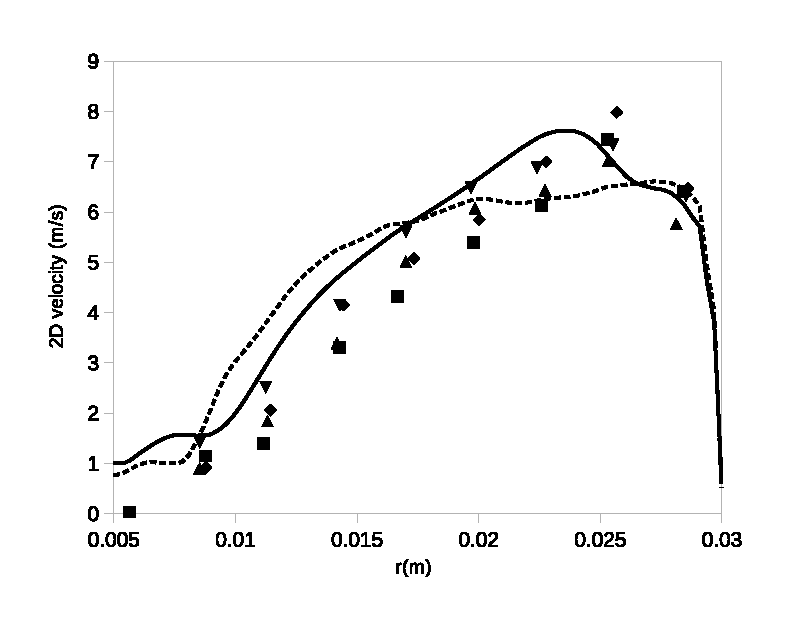
\includegraphics[width=3in]{imgs/nozzle_pump/pump_velblade.eps}\\
    \vspace{.5cm}
    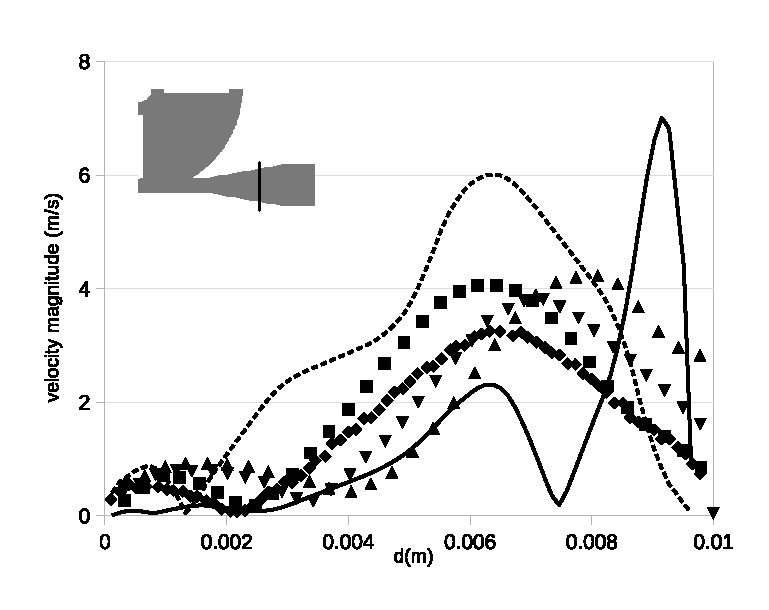
\includegraphics[width=3in]{imgs/nozzle_pump/pump_veldiffuser.eps}
    \caption{The magnitude of the two-dimensional velocity on the xy-plane passing the mid-axis plane of the outlet diffuser with experiments and simulations. Left: along the radial direction from the rotor center in the housing. Right: along the in the outlet diffuser. $\blacktriangledown$ $\blacktriangle$ $\blacksquare$ $\blacklozenge$: experiments \cite{mali_cfd}. Solid line: FEM. Dashed line: PFEM-2. }
    \label{fig:pumpvelprofile}
\end{figure}